% !TEX program = lualatex
\documentclass[border=6pt]{standalone}
% ---------------------------------------------------------------------------
% tikzpreamble.tex -- shared by main.tex and by every standalone in tikz/
% ---------------------------------------------------------------------------
\usepackage{amsmath}
\usepackage{amssymb}
\usepackage{tikz}
\usepackage{circuitikz}
\usetikzlibrary{arrows.meta,calc,positioning,decorations.pathmorphing,decorations.pathreplacing,
                decorations.markings,patterns,angles,quotes,fit,
                shapes.geometric,shapes.misc,backgrounds,intersections}

\ctikzset{bipoles/length=0.85cm}
\ctikzset{resistors/scale=0.85}
\ctikzset{capacitors/scale=0.9}

\tikzset{
  wire/.style      = {line width=0.7pt},
  dashedwire/.style= {line width=0.7pt, densely dashed},
  term/.style      = {circle, draw, line width=0.6pt, fill=white,
                      inner sep=0pt, minimum size=4.5pt},
  node dot/.style  = {circle, fill=black, inner sep=0pt, minimum size=4pt},
  boxlabel/.style  = {font=\sffamily\small},
  annot/.style     = {font=\small, align=left},
  phasor/.style    = {-{Stealth[length=3.2mm,width=2.2mm]}, line width=1.1pt},
  thinphasor/.style= {-{Stealth[length=2.6mm,width=1.8mm]}, line width=0.7pt},
  axis line/.style = {-{Stealth[length=2.6mm,width=1.8mm]}, line width=0.6pt},
  guide/.style     = {densely dashed, line width=0.4pt, gray},
}
\usepackage{siunitx}

\begin{document}
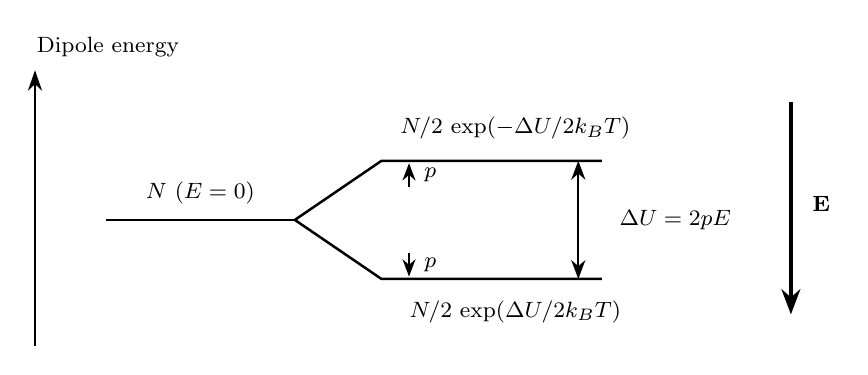
\begin{tikzpicture}[every node/.style={font=\small}]
  \draw[axis line] (0,-1.6) -- (0,1.9);
  \node[anchor=south west,font=\footnotesize] at (-0.1,1.95) {Dipole energy};

  % unsplit level
  \draw[line width=0.9pt] (0.9,0) -- (3.3,0);
  \node[anchor=south,font=\footnotesize] at (2.1,0.08) {$N$ ($E=0$)};

  % splitting
  \draw[line width=0.9pt] (3.3,0) -- (4.4,0.75) -- (7.2,0.75);
  \draw[line width=0.9pt] (3.3,0) -- (4.4,-0.75) -- (7.2,-0.75);
  \node[anchor=south,font=\footnotesize] at (6.1,0.9) {$N/2\,\exp(-\Delta U/2k_BT)$};
  \node[anchor=north,font=\footnotesize] at (6.1,-0.9) {$N/2\,\exp(\Delta U/2k_BT)$};

  % dipole arrows
  \draw[-{Stealth[length=2.2mm]},line width=0.8pt] (4.75,0.42) -- (4.75,0.72);
  \node[anchor=west,font=\footnotesize] at (4.82,0.57) {$p$};
  \draw[-{Stealth[length=2.2mm]},line width=0.8pt] (4.75,-0.42) -- (4.75,-0.72);
  \node[anchor=west,font=\footnotesize] at (4.82,-0.57) {$p$};

  % energy difference
  \draw[{Stealth[length=2.4mm]}-{Stealth[length=2.4mm]},line width=0.6pt]
       (6.9,0.75) -- (6.9,-0.75);
  \node[anchor=west,font=\footnotesize] at (7.3,0) {$\Delta U = 2pE$};

  % field
  \draw[-{Stealth[length=3.2mm]},line width=1.3pt] (9.6,1.5) -- (9.6,-1.2);
  \node[anchor=west,font=\footnotesize] at (9.75,0.2) {$\mathbf{E}$};
\end{tikzpicture}
\end{document}
